% VLDB template version of 2020-03-05 enhances the ACM template, version 1.7.0:
% https://www.acm.org/publications/proceedings-template
% The ACM Latex guide provides further information about the ACM template

\documentclass{article}
\usepackage{listings}
\usepackage[margin=20mm]{geometry}
\usepackage{graphicx}
\usepackage{amsfonts}
\usepackage{amsmath}
\usepackage{physics}
\usepackage{parskip}
\usepackage{enumitem}
\usepackage{cancel}

%% The following content must be adapted for the final version
% paper-specific
\newcommand\vldbdoi{XX.XX/XXX.XX}
\newcommand\vldbpages{XXX-XXX}
% issue-specific
\newcommand\vldbvolume{14}
\newcommand\vldbissue{1}
\newcommand\vldbyear{2020}
% should be fine as it is
\newcommand\vldbauthors{\authors}
\newcommand\vldbtitle{\shorttitle} 
% leave empty if no availability url should be set
\newcommand\vldbavailabilityurl{http://vldb.org/pvldb/format_vol14.html}

\newcommand\oname\operatorname

\newtheorem{theorem}{Teor.}
\newtheorem{definition}{Def.}
\newtheorem{example}{Ej.}
\newtheorem{excercise}{Ejer.}

\begin{document}

% Note to self:
%   "It is never possible to expose anyone to both treatments, and therefore statistical inference would still be needed to asses the \textit{causal inference}.

\textbf{Ex. 1.12.1: }Conditional probability: suppose that if $\theta=1$, then $y$ has a normal distribution with mean $1$ and standard deviation $\sigma$, and if $\theta=2$, then $y$ has a normal distribution with mean $2$ and standard deviation $\sigma$. Also, suppose $\oname{Pr}(\theta=1)=0.5$ and $\oname{Pr}(\theta=2)=0.5$.

\begin{enumerate}[label=\alph*]
	\item For $\theta=2$, write the formula for the marginal probability density for $y$ and sketch it.
	\item What is $\oname{Pr}(\theta=1|y=1)$, again supposing $\sigma=2$?
	\item Describe how the posterior density of $\theta$ changes in shape as $\sigma$ is increased and as it is decreased.
\end{enumerate}

\textbf{Answer:}

The formula for the marginal probability is that of $\mathcal N(\theta,\,\sigma^2)$:
\begin{align*}
	p(y|\theta=2)&=\frac1{\sqrt{2\pi\sigma^2}}\exp\left(-\frac12\left(\frac{x-2}\sigma\right)^2\right).
\end{align*}

As for the sketch, I'm too lazy to do it. It's a bell shape, centered at $2$ and $\sigma$ being half the width at about $0.61$ height. There's an xkcd-looking MatPlotLib plot in Figure \ref{fig:1.12.1}.
\begin{figure}[h]
	\centering
	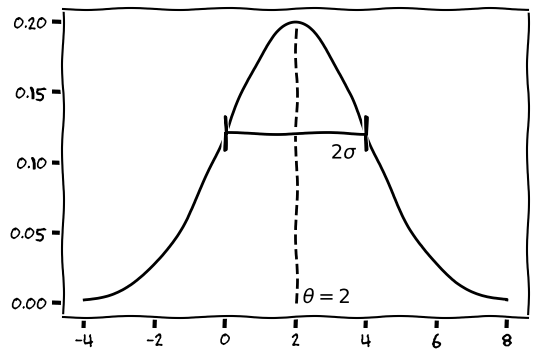
\includegraphics[width=0.4\textwidth]{Numerical/1.12.1}
	\caption{Your typical bell thingy with $\sigma=2$ and mean $2$}
	\label{fig:1.12.1}
\end{figure}

Now then,
\begin{align*}
	\oname{Pr}(\theta=1|y=1)&=\frac{\oname{Pr}(\theta=1)\oname{Pr}(y=1|\theta=1)}{\oname{Pr}(\theta=1)\oname{Pr}(y=1|\theta=1)+\oname{Pr}(\theta=2)\oname{Pr}(y=2|\theta=2)}\\
	&=\frac{0.5\cdot\frac1{\sqrt{8\pi}}}{0.5\cdot\frac1{\sqrt{8\pi}}+0.5\cdot\frac1{\sqrt{8\pi}}\exp\left(-\frac18\right)}\\
	&\approx0.53.
\end{align*}

The posterior for $\theta$ gets more homogeneous as $\sigma$ increases, and instead gets closer to $(1, 0)$ otherwise, since $\sigma$ directly defines the overlap between both likelihood functions as functions of $y$.

\textbf{Ex. 1.12.2: }Conditional means and variances: show that $(1.8)$ and $(1.9)$ hold if $u$ is a vector.

\textbf{Answer:}

No, $u$ are a vector.

Just kidding. Proof of $(1.8)$ is symbolically the same. As to $(1.9)$, it is \textit{about} the same. First, note that
\begin{align*}
	\oname{var}(x)&=\mathrm E\left[\left(x-\mathrm E(x)\right)\left(x-\mathrm E(x)\right)^T\right]\\
	&=\mathrm E\left[\left(x-\mathrm E(x)\right)\left(x^T-\left(\mathrm E(x)\right)^T\right)\right]\\
	&=\mathrm E\left[xx^T-x\left(\mathrm E(x)\right)^T-\mathrm E(x)x^T+\left(\mathrm E(x)\right)\left(\mathrm E(x)\right)^T\right]\\
	&=\mathrm E\left(xx^T\right)-\left(\mathrm E(x)\right)\left(\mathrm E(x)\right)^T.
\end{align*}
The result then follows replacing any occurrence of $x^2$ by $xx^T$.

\textbf{Ex. 1.12.3: }Probability calculation for genetics (from Lindley, 1965): suppose that in each individual of a large population there is a pair of genes, each of which can be either $x$ or $X$, that controls eye color: those with $xx$ have blue eyes, while heterozygotes (those with $Xx$ or $xX$) and those with $XX$ have brown eyes. The proportion of blue-eyed individuals is $p^2$ and of heterozygotes is $2p(1-p)$, where $0<p<1$. Each parent transmits one of its own genes to the child; if a parent is a heterozygote, the probability that it transmits the gene of type $X$ is $\frac12$. Assuming random mating, show that among brown-eyed children of brown-eyed parents, the expected proportion of heterozygotes is $2p/(1+2p)$. Suppose Judy, a brown-eyed child of brown-eyed parents, marries a heterozygote, and they have $n$ children, all brown-eyed. Find the posterior probability that Judy is a heterozygote and the probability that her first grandchild has blue eyes.

\textbf{Answer:}

Denoting $p_1$ and $p_2$ both parents' alleles, random mating implies $p(p_1|p_2)$ and $p(p_2)$ are both given by the population's proportion of people with $p_2$ and $p_1$ after $p_2$. We'll also use the hypothesis of a large pool of people, so that $p$ remains approximately equal after picking one of the parents. We thus have $p(p_1,\,p_2)=p(p_1)\,p(p_2)$.

So, if both parents are brown-eyed, they're one from $\{xX,\,Xx,\,XX\}$. The conditional probability of being any of the first two is
\begin{align*}
	\oname{Pr}(xX+Xx|xX+Xx+XX)&=\frac{\oname{Pr}((xX+Xx)(xX+Xx+XX))}{\oname{Pr}(xX+Xx+XX)}\\
	&=\frac{2p(p-1)}{2p(p-1)+(1-p)^2}\\
	&=\frac{2p}{1+p}.
\end{align*}
And the probability of transmiting either allele is then $1/2$. The probability of being an heterocygote is twice the probability that one of the parent gives $x$ and the other $X$, so
\begin{align*}
	&2\left(\frac12\frac{2p}{1+p}\right)\left(\frac12\frac{2p}{1+p}+\frac{1-p}{1+p}\right)\\
	&2\left(\frac12\frac{2p}{1+p}\right)\left(\frac1{1+p}\right)\\
	&\frac{2p}{(1+p)^2}.
\end{align*}
Finally, since we want this conditioned to the fact that they're all brown eyed, we must quotient this with the probability of being brown eyed, which is the above quantity plus the probability that both parents give $X$, $1/(1+p)^2$, so the final proportion is
\begin{align*}
	&\left[\frac{2p}{(1+p)^2}\right]\left[\frac{2p}{(1+p)^2}+\frac1{(1+p)^2}\right]^{-1}\\
	&=\frac{2p}{2p+1}.
\end{align*}

We are now asked the posterior probability of Judy being heterozygote after blah blah blah. So the priors of them being and not being heterozygote are $2p/(2p+1)$ and $1/(2p+1)$. The likelihood of the $n$ childrens are $\left(\frac34\right)^n$ and $1$ respectively, so that the posterior probability is
\begin{align*}
	\frac{2p}{2p+\left(\frac43\right)^n},
\end{align*}
which of course tends to $0$ as $n$ increases, since the likelihood of not having a blue eyed child decreases as $n$ increases.

\textbf{Ex. 1.12.4: }Probability assignment: we will use the football dataset to estimate some conditional probabilities about professional football games. There were twelve games with point spread of $8$ points; the outcomes in those games were: $-7$, $-5$, $-3$, $-3$, $1$, $6$, $7$, $13$, $15$, $16$, $20$, and $21$, with positive values indicating wins by the favorite and negative values indicating wins by the underdog. Consider the following conditional probabilities:
\begin{align*}
	&\oname{Pr}(\text{favorite wins}|\text{point spread}=8),\\
	&\oname{Pr}(\text{favorite wins by at least $8$}|\text{point spread}=8),\\
	&\oname{Pr}(\text{favorite wins by at least $8$}|\text{point spread}=8\text{ and favorite wins}).
\end{align*}
\begin{enumerate}[label=\alph*]
	\item Estimate each of these using the relative frequencies of games with a point spread of $8$.
	\item Estimate each using the normal approximation for the distribution of $(\text{outcome}-\text{point spread})$.
\end{enumerate}

\textbf{Answer: }

Point a is just counting:
\begin{align*}
	&\oname{Pr}(\text{favorite wins}|\text{point spread}=8)=8/12\approx0.58\\
	&\oname{Pr}(\text{favorite wins by at least $8$}|\text{point spread}=8)=5/12\approx0.42,\\
	&\oname{Pr}(\text{favorite wins by at least $8$}|\text{point spread}=8\text{ and favorite wins})=5/8\approx0.63.
\end{align*}

Point b uses the model $P(\text{wins by $\hat{y}$}|\text{point spread of $x$})=\mathcal N(\hat{y}|x,\,14^2)$, so
\begin{align*}
	\oname{Pr}(\text{favorite wins}|\text{point spread}=8)&=1-\Phi\left(\frac{0-8}{14}\right)\\
	&\approx0.72\\
	\oname{Pr}(\text{favorite wins by at least $8$}|\text{point spread}=8)&=0.5,\\
	\oname{Pr}(\text{favorite wins by at least $8$}|\text{point spread}=8\text{ and favorite wins})&\approx\frac{0.5}{0.72}\\
	&\approx0.69
\end{align*}

\textbf{Ex. 1.12.5: }Probability assignment: the $435$ U.S. Congressmembers are elected to two-year terms; the number of voters in an individual congressional election varies from $50\,000$ to $350\,000$. We will use various sources of information to estimate roughly the probability that at least one congressional election is tied in the next national election.
\begin{enumerate}[label=\alph*]
	\item Use any knowledge you have about U.S. politics. Specify clearly what information you are using to construct this conditional probability, even if your answer is just a guess.
	\item Use the following information: in the period $1900-1992$, there were $20\,597$ congressional elections, out of which $6$ were decided by fewer than $10$ votes and $49$ by fewer than $100$ votes.
\end{enumerate}

\textbf{Answer:}

Got no knowledge. Gonna skip this one.

\textbf{Ex. 1.12.6: }Conditional probability: approximately $1/125$ of all births are fraternal twins and $1/300$ of births are identical twins. Elvis Presley had a twin brother (who died at birth). What is the probability that Elvis was an identical twin? (You may approximate the probability of a boy or girl birth as $1/2$).

\textbf{Answer:}

We need
\begin{align*}
	P(\text{Identical}|\text{Both male})&=\frac{P(\text{Both male}|\text{Identical})P(\text{Identical})}{P(\text{Both male}|\text{Identical})P(\text{Identical})+P(\text{Both male}|\text{Fraternal})P(\text{Fraternal})}.
\end{align*}

This is pretty straightforward:
\begin{align*}
	P(\text{Both male}|\text{Identical})&=\frac12,\\
	P(\text{Identical})&=\frac1{300},\\
	P(\text{Both male}|\text{Fraternal})&=\frac12\frac12,\\
	P(\text{Fraternal})&=\frac1{125}
\end{align*}

It then follows that
\begin{align*}
	P(\text{Identical}|\text{Both male})&=5/11\approx0.45.
\end{align*}

\textbf{Ex. 1.12.7: }Conditional probability: the following problem is loosely based on the television game show \textit{Let's Make a Deal}. At the end of the show, a contestant is asked to choose one of three large boxes, where one box contains a fabulous prize and the other two boxes contain lesser prizes. After the contestant chooses a box, Monty Hall, the host of the show, opens one of the two boxes containing smaller prizes. (In order to keep the conclusion suspenseful, Monty does not open the box selected by the contestant.) Monty offers the contestant the opportunity to switch from the chosen box to the remaining unopened box. Should the contestant switch or stay with the original choice? Calculate the probability that the contestant wins under each strategy. This is an exercise in being clear about the information that should be conditioned on when constructing a probability judgement.

\textbf{Answer:}

Let $W_i=\text{the winning box is the $i$th}$, $P_i=\text{the player chose the $i$th box}$, $H_i=\text{the host opened the $i$th box}$. We then want
\begin{align*}
	P(W_1|P_2H_3)&=\frac{P(H_3|P_2W_1)P(W_1|P_2)}{P(H_3|P_2W_1)P(W_1|P_2)+P(H_3|P_2W_2)P(W_2|P_2)+P(H_3|P_2W_3)P(W_1|P_3)}\\
	&=\frac{1}{1+\frac12+0}\\
	&=\frac23.
\end{align*}

So, the obvious choice is to switch.

\textbf{Ex. 1.12.8: }Subjective probability: discuss the following statement. `The probability of event $E$ is considered ``subjective'' if two rational persons $A$ and $B$ can assign unequal probabilities to $E$, $P_A(E)$ and $P_B(E)$. These probabilities can also be interpreted as ``conditional'': $P_A(E)=P(E|I_A)$ and $P_B(E)=P(E|I_B)$, where $I_A$ and $I_B$ represent the knowledge available to persons $A$ and $B$, respectively'. Apply this idea to the following examples.
\begin{enumerate}[label=\alph*]
	\item The probability that a `$6$' appears when a fair die is rolled, where $A$ observes the outcome of the die roll and $B$ does not.
	\item The probability that Brazil wins the next World Cup, where $A$ is ignorant of soccer and $B$ is a knowledgeable sports fan.
\end{enumerate}

\textbf{Answer:}

I'd say both are subjective. The knowledge of the die throw \textit{before} observation is that there's $1/6$ probability for any side, since it's a fair die. But if $A$ knows the result of the die, then the probability distribution should no longer incorporate any uncertainty. The second example is more evident, since it is expected that people more knowledgeable have a better understanding of their degree of knowledge.

\textbf{Ex. 1.12.9: }Simulation of a queuing problem: a clinic has three doctors. Patients come into the clinic at random, starting at $9$ a.m., according to a Poisson process with time parameter $10$ minutes: that is, the time after opening at which the first patient appears follows an exponential distribution with expectation $10$ minutes and then, after each patient arrives, the waiting time until the next patient is independently exponentially distributed, also with expectation $10$ minutes. When a patient arrives, he or she waits until a doctor is available. The amount of time spent by each doctor with each patient is a random variable, uniformly distributed between $5$ and $20$ minutes. The office stops admitting new patients at $4$ p.m. and closes when the last patient is through with the doctor.
\begin{enumerate}[label=\alph*]
	\item Simulate this process once. How many patients came to the office? How many had to wait for a doctor? What was their average wait? When did the office close?
	\item Simulate the process $100$ times and estimate the median and $50\%$ interval for each of the summaries in $(a)$.
\end{enumerate}

\textbf{Answer:}

Script ``1.12.9.py'' generates these answers:
\input{Numerical/1.12.9.out}

The rest of answers can be found in Figure \ref{fig:1.12.9}.
\begin{figure}[h]
	\centering
	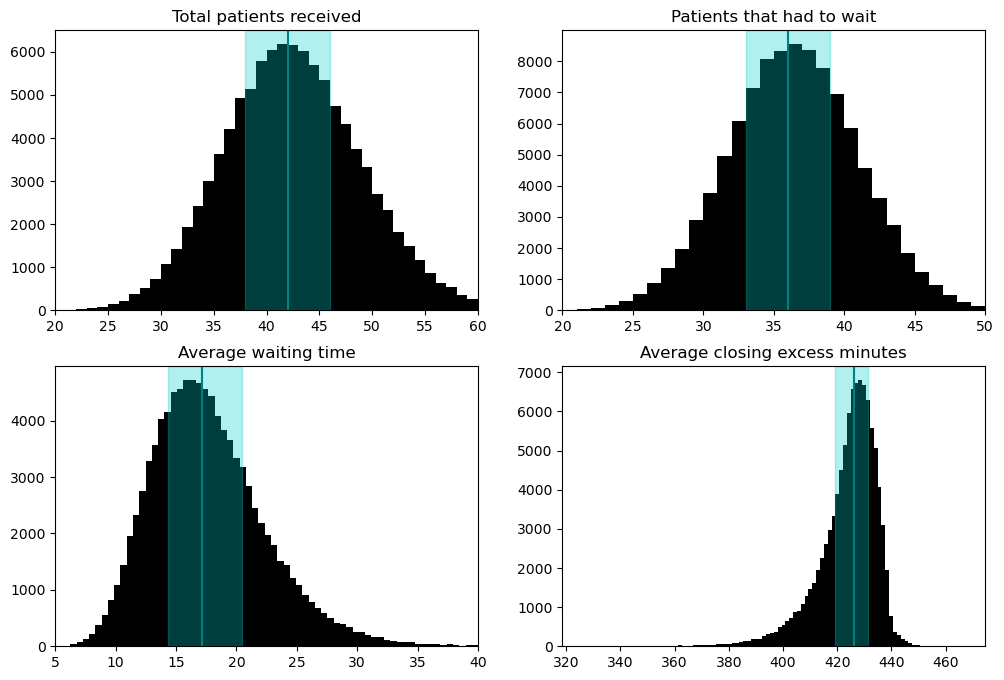
\includegraphics[width=0.8\textwidth]{Numerical/1.12.9}
	\caption{Histograms for the stuff after $100000$ runs.}
	\label{fig:1.12.9}
\end{figure}

\textbf{Ex. 2.11.1: }Posterior inference: suppose you have a $\oname{Beta}(4,\,4)$ prior distribution on the probability $\theta$ that a coin will yield a `head' when spun in a specified manner. The coin is independently spun ten times, and `heads' appear fewer than $3$ times. You are not told how many heads were seen, only that the number is less than $3$. Calculate your exact posterior density (up to a proportionality constant) for $\theta$ and sketch it.

\textbf{Answer:}

We are asked
\begin{align*}
	p(\theta|y<3)&=p(\theta|(y=0)+(y=1)+(y=2))\\
	&\propto p((y=0)+(y=1)+(y=2)|\theta)p(\theta)\\
	&=(p(y=0|\theta)+p(y=1|\theta)+p(y=2|\theta))p(\theta).
\end{align*}
Each term separately will yield $\oname{Beta}(4+y,\,4+(10-y))$, so that the final probability distribution is plainly
\begin{align*}
	\frac13\left[\oname{Beta}(4,\,14)+\oname{Beta}(5,\,13)+\oname{Beta}(6,\,12)\right].
\end{align*}
Those have means $4/18$, $5/18$, $6/18$, so that the mean is $5/18$. More concretely, if
\begin{align*}
	p(x)&=\sum_iw_ip_i(x),
\end{align*}
then the expectation of stuff is given by
\begin{align*}
	\mathrm E\cdot&=\int\mathrm dx\;p(x)\cdot\\
	&=\sum_iw_i\int\mathrm dx\;p_i(x)\cdot\\
	&=\sum_iw_i\mathrm E_i\cdot.
\end{align*}

It then follows that
\begin{align*}
	\mathrm E\theta&=\frac13\left[\mathrm E_1\theta+\mathrm E_2\theta+\mathrm E_3\theta\right]\\
	&=\frac5{18}.
\end{align*}
The same proccess can yield the new variance.

The corresponding computer graph is shown in Figure \ref{fig:2.11.1}.
\begin{figure}[h]
	\centering
	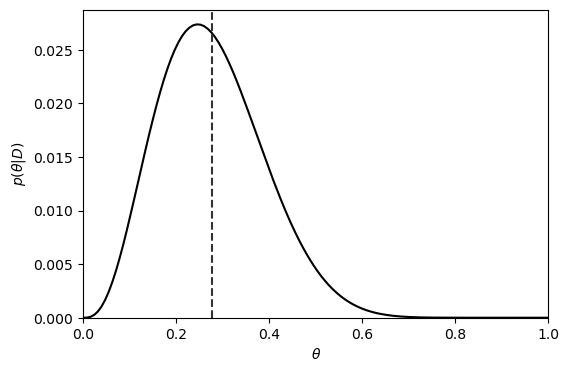
\includegraphics[width=0.6\textwidth]{Numerical/2.11.1}
	\caption{Probability distribution for $\theta$ given the number of heads is less than $3$.}
	\label{fig:2.11.1}
\end{figure}

\textbf{Ex. 2.11.2: }Predictive distributions: consider two coins, $C_1$ and $C_2$, with the following characteristics: $\oname{Pr}(\text{heads}|C_1)=0.6$ and $\oname{Pr}(\text{heads}|C_2)=0.4$. Choose one of the coins at random and imagine spinning it repeatedly. Given that the first two spins from the chosen coin are tails, what is the expectation of the number of additional spins until a head shows up?

\textbf{Answer:}

Here I'll represent the data by $D$.

The conditional probability that we make $n$ tosses until heads is found is
\begin{align*}
	p(n|C_i)&=\left(\oname{Pr}(\text{tails}|C_i)\right)^{n-1}\oname{Pr}(\text{heads}|C_i),
\end{align*}
so that
\begin{align*}
	p(n|D)&=\sum_ip(n,\,C_i|D)\\
	&=\sum_ip(n|C_i)\oname{Pr}(C_i|D).
\end{align*}
Since we have no information as to which coin we picked, we'll take $\oname{Pr}(C_i)=\frac12$ which, together with $\oname{Pr}(D|C_i)=\left(\oname{Pr}(\text{tails}|C_i)\right)^2$ yield $\oname{Pr}(C_i|D)=\left(\oname{Pr}(\text{tails}|C_i)\right)^2/\left[\left(\oname{Pr}(\text{tails}|C_i)\right)^2+\left(\oname{Pr}(\text{tails}|C_{\overline{i}})\right)^2\right]$, where $\overline{i}$ is not $i$. Numerically, this yields $P(C_2|D)=0.69$, nice.

Anyways, we also have $p(n|C_i)=\left(\oname{Pr}(\text{tails}|C_i)\right)^{n-1}\oname{Pr}(\text{heads}|C_i)$, so we get our final result of
\begin{align*}
	p(n|D)&=\frac{\left(\oname{Pr}(\text{tails}|C_1)\right)^{n+1}\oname{Pr}(\text{heads}|C_1)+\left(\oname{Pr}(\text{tails}|C_2)\right)^{n+1}\oname{Pr}(\text{heads}|C_2)}{\left(\oname{Pr}(\text{tails}|C_1)\right)^2+\left(\oname{Pr}(\text{tails}|C_2)\right)^2}.
\end{align*}

Our final calculation is then $\mathrm E[n]=\sum_{n=1}np(n)$, which can be done analitically just fine but I wont, and yields about $2.24$.

\textbf{Ex. 2.11.3: }Predictive distributions: let $y$ be the number of $6$'s in $1000$ rolls of a fair die.
\begin{enumerate}[label=\alph*]
	\item Sketch the approximate distribution of $y$, based on the normal approximation.
	\item Using the normal distribution table, give approximate $5\%$, $25\%$, $50\%$, $75\%$ and $95\%$ points for the distribution of $y$.
\end{enumerate}

\textbf{Answer:}

We have $y\sim\oname{B}(1000,\,1/6)$, with mean $166.\overline{6}$ and deviation $11.8$. So I should draw a bell curve which should have a width of $23.6$ at $0.6$ its height, centered in $166.6$. As for the table thingy, the following Python interpreter run has been performed
\begin{lstlisting}[language=Python]
In [1]: import scipy.stats as st

In [2]: [ 166.6+11.8*st.norm.ppf(x) for x in [0.05, 1/4, 1/2, 3/4, 0.95] ]
Out[2]:
[147.1907272019726,
 158.64102094768623,
 166.6,
 174.55897905231376,
 186.00927279802738]
\end{lstlisting}

\textbf{Ex. 2.11.4: }Predictive distributions: let $y$ be the number of $6$'s in $1000$ independent rolls of a particular real die, which may be unfair. Let $\theta$ be the probability that the die lands on `$6$'.

Suppose your prior distribution for $\theta$ is as follows:
\begin{align*}
	\oname{Pr}(\theta=1/12)&=0.25\\
	\oname{Pr}(\theta=1/6)&=0.5\\
	\oname{Pr}(\theta=1/4)&=0.25.
\end{align*}

\begin{enumerate}[label=\alph*]
	\item Using the normal approximation for the conditional distributions, $p(y|\theta)$, sketch your approximate prior predictive distribution for $y$.
	\item Give approximate $5\%$, $25\%$, $50\%$, $75\%$, and $95\%$ points for the distribution of $y$. (Be careful here: $y$ does not have a normal distribution, but you can still use the normal distribution as part of your analysis.)
\end{enumerate}

\textbf{Answer:}

Again we have $p(y)=\sum_\theta p(y|\theta)p(\theta)$. Under the normal approximation, $y|\theta\sim\mathcal N(n\theta,\,n\theta(1-\theta))$, so we'll have
\begin{align*}
	y|\theta\sim 0.25\cdot N(83.3,\,8.74^2)+0.5\cdot N(166.7,\,11.8^2)+0.25\cdot N(250, 13.7),
\end{align*}
which is a pretty disjoint (and thus easily drawable) mixture if you ask me.
\begin{figure}[h]
	\center
	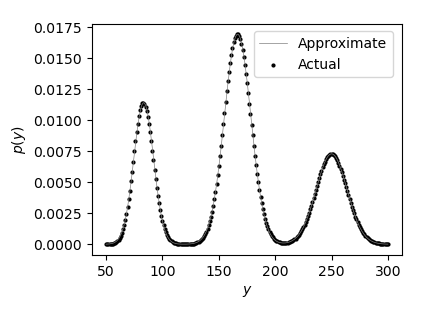
\includegraphics[width=0.4\textwidth]{Numerical/2.11.4.png}
	\caption{Actual and normally-approximated predictive prior distribution for $y$}
	\label{fig:2.11.4}
\end{figure}

As for the approximate points, we can essentially regard the distributions as disjoint, so that the $5\%$ point is the $20\%$ of the first one, the $25\%$ can be approximated as, say, the middle point between the first two Gaussians, the $50\%$ point as the mean $166.7$ of the middle Gaussian, and so on. So, \textit{a ojo}, they should be about $70$, $120$, $167$, $210$, and $270$. But I shall put this handwavery to the test via numerical integration, which is performed in the script `2.11.4.py'. For the real values it yields $76$, $120$, $167$, $207$, and $261$. For the normal-plus-disjointness-approximated values we get $76$, $125$, $167$, $208$, and $262$.

\textbf{Ex. 2.11.5: }Posterior distribution as a compromise between prior information and data: let $y$ be the number of heads in $n$ spins of a coin, whose probability of heads is $\theta$.
\begin{enumerate}[label=\alph*]
	\item If your prior distribution for $\theta$ is uniform on the range $[0,\,1]$, derive your prior predictive distribution for $y$,
		\begin{align*}
			\oname{Pr}(y=k)&=\int_0^1\oname{Pr}(y=k|\theta)\mathrm d\theta,
		\end{align*}
		for each $k=0,\,1,\,\ldots,\,n$.
	\item Suppose you assign a $\oname{Beta}(\alpha,\,\beta)$ prior distribution for $\theta$, and then you observe $y$ heads out of $n$ spins. Show algebraically that your posterior mean of $\theta$ always lies between your prior mean, $\frac{\alpha}{\alpha+\beta}$, and the observed relative frequency of heads, $\frac{y}n$.
	\item Show that, if the prior distribution on $\theta$ is uniform, the posterior variance of $\theta$ is always less than the prior variance.
	\item Give an example of a $\oname{Beta}(\alpha,\,\beta)$ prior distribution and data $y,\,n$, in which the posterior variance of $\theta$ is higher than the prior variance.
\end{enumerate}

\textbf{Answer:}

Point a:
\begin{align*}
	\oname{Pr}(y=k)&=\int_0^1\mathrm d\theta\;\oname{Pr}(y=k|\theta)\\
	&=\int_0^1\mathrm d\theta\;\begin{pmatrix}n\\k\end{pmatrix}\theta^k(1-\theta)^{n-k}\\
	&=\begin{pmatrix}n\\k\end{pmatrix}\int_0^1\mathrm d\theta\;\theta^k(1-\theta)^{n-k}\\
	&=\begin{pmatrix}n\\k\end{pmatrix}\left\{\cancelto{0}{\left[\frac1{k+1}\theta^{k+1}(1-\theta)^{n-k}\right]_0^1}+\frac{n-k}{k+1}\int_0^1\mathrm d\theta\;\theta^{k+1}(1-\theta)^{n-k-1}\right\}\\
	&=\begin{pmatrix}n\\k\end{pmatrix}\frac{n-k}{k+1}\frac{n-k-1}{k+2}\ldots\frac{1}{n}\int_0^1\mathrm d\theta\;\theta^n\\
	&=\begin{pmatrix}n\\k\end{pmatrix}\frac{k!(n-k)!}{(n+1)!}\\
	&=\frac{1}{n+1}.
\end{align*}

Point b:

We've seen in the book that we now have $\theta|y\sim\oname{Beta}(y+\alpha,\,n-y+\beta)$, which has expectation value
\begin{align*}
	\frac{y+\alpha}{n+\alpha+\beta}&=\frac{y}{n}\frac{n}{n+\alpha+\beta}+\frac\alpha{\alpha+\beta}\frac{\alpha+\beta}{n+\alpha+\beta}\\
	&=w\frac{y}n+(1-w)\frac\alpha{\alpha+\beta}\;\;\left(w=\frac{n}{n+\alpha+\beta}\in[0,\,1]\right).
\end{align*}
This is a linear function of $w$ which goes from $\frac{y}n$ to $\frac\alpha{\alpha+\beta}$ as $w$ goes from $0$ to $1$, thus proving the result.

Point c:

Since $\theta\sim1$, its variance is
\begin{align*}
	\int_0^1\mathrm d\theta\;\left(\theta-\frac12\right)^2&=\frac13\left[\left(\theta-\frac12\right)^3\right]_0^1\\
	&=\frac1{12}.
\end{align*}
Now, $\theta|y\sim\oname{Beta}(y+1,\,n-y+1)$, which has variance
\begin{align*}
	\frac{(y+1)(n-y+1)}{(n+2)^2(n+3)}.
\end{align*}
As a function of $y$, this is proportional to the denominator $-y^2+ny+n+1$, whose maximum is at $\frac12n$ and yields $\frac14\left(2n+1\right)$, so that
\begin{align*}
	\frac{(y+1)(n-y+1)}{(n+2)^2(n+3)}&\leq\frac14\frac{\left(2n+1\right)^2}{\left(n+2\right)^2(n+3)}.
\end{align*}
This function can be maximized analitically via derivation, but I just plotted it. It's maximum is around $3$, taking the value $49/600<50/600=1/12$. Such a close call though.

As for point $c$, take $\oname{Beta}(3,\,1)$, yielding variance $0.0375$, and suppose one negative outcome is measured, taking the posterior distribution towards $\oname{Beta}(3,\,2)$ with variance $0.04$.

\textbf{Ex. 2.11.6: }Predictive distributions: Derive the mean and variance ($2.17$) of the negative binomial predictive distribution for the cancer rate example, using the mean and variance formulas ($1.8$) and ($1.9$).

\textbf{Answer:}

Formulas ($1.8$) and ($1.9$) are
\begin{align*}
	\mathrm E(u)&=\mathrm E(\mathrm E(u|v)),\\
	\mathrm{var}(u)&=\mathrm E(\mathrm{var}(u|v))+\mathrm{var}(\mathrm E(u|v)).
\end{align*}

We're thus asked the mean and variance of the distribution $p(y)=\int\mathrm d\theta\;p(y|\theta)p(\theta)$, where $\theta\sim\oname{Gamma}(\alpha,\,\beta)$ and $y|\theta\sim\oname{Poisson}(10n\theta)$. Direct application follows:
\begin{align*}
	\mathrm E(y)&=\mathrm E(\mathrm E(y|\theta))\\
	&=\mathrm E(10n\theta)\\
	&=10n_j\mathrm E(\theta)\\
	&=10n\frac\alpha\beta.\\
	\mathrm{var}(y)&=\mathrm E(\mathrm{var}(y|\theta))+\mathrm{var}(\mathrm E(y|\theta))\\
	&=\mathrm E(10n\theta)+\mathrm{var}(10n\theta)\\
	&=10n\frac\alpha\beta+(10n)^2\frac\alpha{\beta^2},
\end{align*}
where the mean and variance of the $\oname{Gamma}$ and $\oname{Poisson}$ have been Googled and used straight away.

\textbf{Ex. 2.11.7: }Noninformative prior densities:
\begin{enumerate}[label=\alph*]
	\item For the binomial likelihood, $y\sim\oname{Bin}(n,\,\theta)$, show that $p(\theta)\propto\theta^{-1}(1-\theta)^{-1}$ is the uniform prior distribution for the natural parameter of the exponential family.
	\item Show that if $y=0$ or $n$, the resulting posterior distribution is improper.
\end{enumerate}

\textbf{Answer:}

We can express the binomial likelihood in exponential form as follows
\begin{align*}
	\oname{Bin}(y|n,\,\theta)&=\begin{pmatrix}n\\y\end{pmatrix}\theta^y(1-\theta)^{n-y}\\
	&=\begin{pmatrix}n\\y\end{pmatrix}(1-\theta)^n\left(\frac\theta{1-\theta}\right)^y\\
	&=\begin{pmatrix}n\\y\end{pmatrix}(1-\theta)^n\exp\left(y\log\left(\frac\theta{1-\theta}\right)\right).
\end{align*}
It then becomes clear that the natural parameter is $\phi=\log\left(\frac\theta{1-\theta}\right)$. Since the transformation between $\phi$ and $\theta$ is one-to-one,
\begin{align*}
	p(\phi)&=p(\theta)\abs{\frac{\mathrm d\phi}{\mathrm d\theta}}^{-1}\\
	&=\theta^{-1}(1-\theta)^{-1}\abs{\frac{\theta}{1-\theta}\left(1-\theta\right)^2}\\
	&=1.
\end{align*}

As for the posterior distribution, we have
\begin{align*}
	p(\theta|y)&\propto p(y|\theta)p(\theta)\\
	&\propto\theta^{y-1}(1-\theta)^{n-y-1}.
\end{align*}
Whether $y=0$ or $y=n$ we have something of the form $\eta^{-1}(1-\eta)^{n-1}$, $\eta$ being either $\theta$ or $1-\theta$, so that the integral of this quantity over $\eta$ is precisely the normalization required, but it yields
\begin{align*}
	\int_0^1\mathrm d\eta\;\eta^{-1}(1-\eta)^{n-1}&=\int_0^1\mathrm d\eta\;\sum_{k=0}^{n-1}\begin{pmatrix}n-1\\k\end{pmatrix}\eta^{-1}\eta^k\\
	&=\sum_{k=0}^{n-1}\begin{pmatrix}n-1\\k\end{pmatrix}\int_0^1\mathrm d\eta\;\eta^{k-1}\\
	&=\int_0^1\mathrm d\eta\;\eta^{-1}+\sum_{k=1}^{n-1}\begin{pmatrix}n-1\\k\end{pmatrix}\int_0^1\mathrm d\eta\;\eta^{k-1}\\
	&=\infty+\text{something finite},
\end{align*}
whence this integral is improper.

\textbf{Ex. 2.11.8: }Normal distribution with unknown mean: a random sample of $n$ students is drawn from a large population, and their weights are measured. The average weight of the $n$ sampled students is $\bar{y}=150\text{ pounds}$. Assume the weights in the population are normally distributed with unknown mean $\theta$ and known standard deviation $20\text{ pounds}$. Suppose your prior distribution for $\theta$ is normal with mean $180$ and standard deviation $40$.
\begin{enumerate}[label=\alph*]
	\item Give your posterior distribution for $\theta$. (Your answer will be a function of $n$.)
	\item A new student is sampled at random from the same population and has a weight of $\tilde{y}\text{ pounds}$. Give a posterior predictive distribution for $\tilde{y}$. (Your answer will still be a function of $n$.)
	\item For $n=10$, give a $95\%$ posterior interval for $\theta$ and a $95\%$ posterior predictive interval for $\tilde{y}$.
	\item Do the same for $n=100$.
\end{enumerate}

\textbf{Answer:}

By hypothesis, $y|\theta\sim\oname{N}(\theta,\,20^2)$ and $\theta\sim\oname{N}(180,\,40^2)$, so that $\bar{y}|\theta\sim\oname{N}(\theta,\,20^2/n)$, and thus $\theta|\bar{y}$ is gonna be given by a normal distribution with
\begin{align*}
	\mathrm E(\theta|\bar{y})&=\frac{40^{-2}180+n20^{-2}150}{40^{-2}+n20^{-2}},\\
	\mathrm{var}(\theta|\bar{y})&=\frac1{40^{-2}+n20^{-2}}.
\end{align*}
I could put some numbers there, but it'd be no use. I instead ploted probability desntiy for $\theta|\bar{y}$ (vertical axis) as a function of sample size $n$ (horizontal axis) for $n$ between $0$ and $100$, as shown in Figure \ref{fig:2.11.8}.
\begin{figure}[h]
	\center
	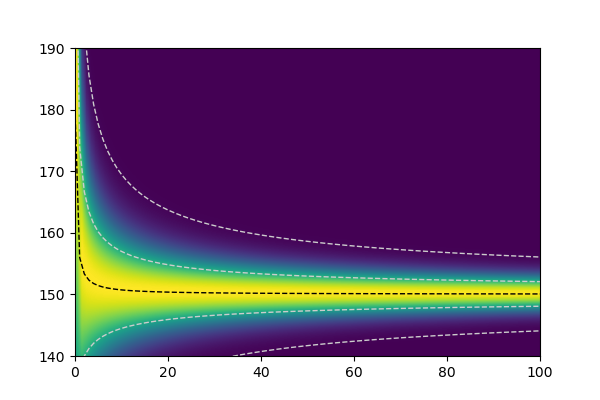
\includegraphics[width=0.5\textwidth]{Numerical/2.11.8.png}
	\caption{Non-normalized probability distribution for $\theta|\bar{y}$ as a function of $\theta$ and number of samples $n$. Black contour is the mean, and grey contours are $1$ and $3$ standard deviations from it.}
	\label{fig:2.11.8}
\end{figure}

Since the actual precision of the data is so small, the mean converges quickly towards the observed mean.

The posterior predictive distribution is the same, but incorporates an extra $20$ in the standard deviation. In particular, for $n=10$, the posterior probabilities for $\theta$ and $\tilde{y}$ have mean $150.73$ and respectively a standard deviation of $6.24$ and $26.24$, so that the $\sim95\%$ intervals are $150.73\pm12.48$ and $150.73\pm42.48$. For $n=100$, the mean becomes $150.07$ and the standard deviations $1.99$ and $20.199$, so that the intervals are $150.07\pm4$ and $150.07\pm48$.

\textbf{Ex. 2.11.9: }Setting parameters for a beta prior distribution: suppose your prior distribution for $\theta$, the proportion of Californians who support the death penalty is beta with mean $0.6$ and standard deviation $0.3$.
\begin{enumerate}[label=\alph*]
	\item Determine the parameters $\alpha$ and $\beta$ of your prior distribution. Sketch the prior density function.
	\item A random sample of $1000$ Californians is taken, and $65\%$ support the death penalty. What are your posterior mean and variance for $\theta$? Draw the posterior density function.
	\item Examine the sensitivity of the posterior distribution to different prior means and widths including a non-informative prior.
\end{enumerate}

\textbf{Answer:}

We equate the mean and the variance
\begin{align*}
	\frac\alpha{\alpha+\beta}&=\mu,\\
	\frac{\alpha\beta}{(\alpha+\beta)^2(\alpha+\beta+1)}&=\sigma^2.
\end{align*}
Replacing $\alpha/(\alpha+\beta)=\mu$ and $\beta/(\alpha+\beta)=1-\mu$ in the second equation yields
\begin{align*}
	\alpha+\beta&=\frac{\mu\left(1-\mu\right)}{\sigma^2}-1,
\end{align*}
which into the first equation implies
\begin{align*}
	\alpha&=\mu\left(\frac{\mu\left(1-\mu\right)}{\sigma^2}-1\right),\\
	\beta&=(1-\mu)\left(\frac{\mu\left(1-\mu\right)}{\sigma^2}-1\right).
\end{align*}

Upon replacing the particular values $\mu=0.6$ and $\sigma=0.3$, we get
\begin{align*}
	\alpha=1,\;\;\beta=\frac23.
\end{align*}

Now, after the sensus we get $650$ positives and $350$ negatives, whence we'll have $\theta|\text{D}\sim\oname{Beta}(650+1, 350+\frac23)$, with mean $65.0\%$ and standard deviation $1.4\%$.

The following table, calculated in the corresponding script to this exercise, evaluates a few alternatives for $\sigma$, ranging from \textit{whoa} prior certainty to complete prior uncertainty.
\input{Numerical/2.11.9.out}

The noninformative alternative diminishes the posterior mean because it's centered around $50\%$ instead of $60\%$, so that it's ``pulling effect'' is more evident.

\textbf{Ex. 2.11.10: }Discrete sample spaces: suppose there are $N$ cable cars in San Francisco, numbered sequentially from $1$ to $N$. You see a cable car at random, it is numbered $203$. You wish to estimate $N$.
\begin{enumerate}[label=\alph*]
	\item Assume your prior distribution on $N$ is geometric with mean $100$; that is,
		\begin{align*}
			p(N)&=(1/100)(99/100)^{N-1},\;\;\text{for }N=1,2,...
		\end{align*}
	      What is your posterior distribution for $N$?
      \item What are the posterior mean and standard deviation of $N$?
      \item Choose a reasonable `noninformative' prior distribution for $N$ and give the resulting posterior distribution, mean, and standard deviation for $N$.
\end{enumerate}

\textbf{Answer:}

Let $q=99/100$. My first instinct was proposing an homogeneous sampling distribution for the number $y$ of the observed cable car, $p(y|N)=1/N$. But this conveys no information on the relation between $y$ and $N$, and thus serves no good.

% TODO: Finish this

\textbf{Ex. 2.11.11: }Computing with a nonconjugate single parameter model: suppose $y_1,\ldots,y_5$ are independent samples from a Cauchy distribution with unknown center $\theta$ and known scale $1$: $p(y_i|\theta)\propto1/(1+(y_i-\theta)^2)$. Assume for simplicity that the prior distribution for $\theta$ is uniform on $[0,\,100]$. Given the observations $(y_1,\ldots,y_5)=(43,\,44,\,45,\,46.5,\,47.5)$:
\begin{enumerate}[label=\alph*]
	\item Compute the unnormalized posterior density function, $p(\theta)p(y|\theta)$, on a grid of points $\theta=0,\,\frac1m,\,\frac2m,\ldots,\,100$, for some large integer $m$. Using the grid approximation, compute and plot the normalized posterior density function, $p(\theta|y)$, as a function of $\theta$.
	\item Sample $1000$ draws of $\theta$ from the posterior density and plot a histogram of the draws.
	\item Use the $1000$ samples of $\theta$ to obtain $1000$ samples from the predictive distribution of a future observation, $y_6$, and plot a histogram of the predictive draws.
\end{enumerate}

\textbf{Answer:}

The following is an excerpt from the script ``2.11.11.py'' that does the math before plotting
\begin{lstlisting}[language=Python]
import numpy as np

def normalized(arr):
    return arr/arr.sum()

m = 2**12 # This is unnecessarily big I guess

y = np.array([43, 44, 45, 46.5, 47.5])
theta = np.linspace(0, 100, m+1)
b_y, b_theta = np.meshgrid(y, theta) # "Big y, big theta"

theta_updf = 1
y_gvn_theta_updf = 1/np.prod(1+(b_y-b_theta)**2, axis=1)
# item a:
theta_gvn_y_pdf = normalized(theta_updf*y_gvn_theta_updf)

np.random.seed(42)

# item b:

def draw_samples(vals, pdf, size=1):
    cdf = np.cumsum(pdf)
    udraws = np.random.uniform(size=size)
    b_cdf, b_udraws = np.meshgrid(cdf, udraws)
    ids = np.argmax(b_cdf > b_udraws, axis=1)
    return vals[ids]

theta_gvn_y_samples = draw_samples(theta, theta_gvn_y_pdf, size=1000)

# item c:
y_pred_samples = np.random.standard_cauchy(size=1000)+theta_gvn_y_samples
\end{lstlisting}

From these data, Figure \ref{fig:2.11.11} is constructed.
\begin{figure}[h]
	\center
	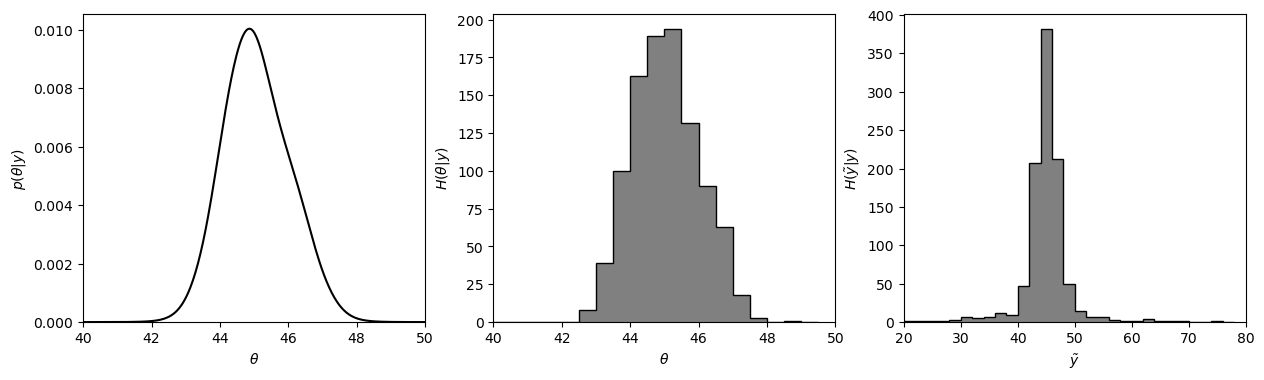
\includegraphics[width=\textwidth]{Numerical/2.11.11.png}
	\caption{Binned approximation to the posterior distribution for $\theta$ (a), histogram from such a distribution (b), and histogram for the posterior predictive distribution for $y_6=\tilde{y}$ (c).}
	\label{fig:2.11.11}
\end{figure}

\textbf{Ex. 2.11.12: }Jeffreys' prior distributions: suppose $y|\theta\sim\oname{Poisson}(\theta)$. Find Jeffreys' prior density for $\theta$, and then find $\alpha$ and $\beta$ for which the $\oname{Gamma}(\alpha,\,\beta)$ density is a close match to Jeffreys' density.

\textbf{Answer:}

Jeffreys prescribes
\begin{align*}
	p(\theta)&\propto\left[J(\theta)\right]^{\frac12},
\end{align*}
where $J(\theta)$ is the Fisher Information for $\theta$:
\begin{align*}
	J(\theta)&=\mathrm E\left(\left(\partial_\theta\log p(y|\theta)\right)^2\middle|\theta\right)=-\mathrm E\left((\partial_\theta)^2\log p(y|\theta)\middle|\theta\right).
\end{align*}

Direct calculation follows:
\begin{align*}
	p(y|\theta)&=\oname{Poisson}(\theta)\\
	&=\frac{\theta^y\mathrm e^{-y}}{y!},\\
	\log p(y|\theta)&=y\log\theta+f(y),\\
	\partial_\theta\log p(y|\theta)&=\frac{y}\theta,\\
	J(\theta)&=\frac1{\theta^2}\mathrm E\left(y^2\right).
\end{align*}

It thus follows that Jeffreys' prior is the improper distribution $p(\theta)\propto1/\theta$.

Since
\begin{align*}
	\oname{Gamma}(\theta|\alpha,\,\beta)&\propto\theta^{\alpha-1}\mathrm e^{-\beta\theta},
\end{align*}
it follows that $\alpha\rightarrow0^+$ and $\beta\rightarrow0^+$ should approach this distribution.

\textbf{Ex. 2.11.13: }Discrete data: Table \ref{table:2.11.13} gives the number of fatal accidents and deaths on scheduled airline flights per year over a ten-year period. We use these data as a numerical example for fitting discrete data models.
\begin{enumerate}[label=\alph*]
	\item Assume that the numbers of fatal accidents in each year are independent with a $\oname{Poisson}(\theta)$ distribution. Set a prior distribution for $\theta$ and determine the posterior distribution based on the data from $1976$ through $1985$. under this model, give a $95\%$ predictive interval for the number of fatal accidents in $1986$. You can use the normal approximation to the gamma and Poisson or compute using simulation.
	\item Assume that the numbers of fatal accidents in each year are independent with a $\oname{Poisson}(\theta)$ distributions with a constant rate and an exposure in each year proportional to the number of passenger miles flown. Set a prior distribution for $\theta$ and determine the posterior distribution based on the data for $1976--1985$ . (Estimate the number of passenger miles flown in each year by dividing the appropriate columns of Table \ref{table:2.11.13} and ignoring round-off errors.) Give a $95\%$ predictive interval for the number of fatal accidents in $1986$ under the assumption that $8\times10^{11}$ passenger miles are flown that year.
	\item Repeat (a) above, replacing `fatal accidents' with `passenger deaths.'
	\item Repeat (b) above, replacing `fatal accidents' with `passenger deaths.'
	\item In which of the cases (a)--(d) above does the Poisson model seem more or less reasonable? Why? Discuss based on general principles, without sepecific reference to the numbers in Table \ref{table:2.11.13}
\end{enumerate}

Incidentally, in $1986$, there were $22$ fatal accidents, $546$ passenger deaths, and a death rate of $0.06$ per $100$ million miles flown. We return to this example in Exercises $3.12$, $6.2$, $6.3$, and $8.14$.

\begin{table}
\begin{center}
\begin{tabular}{ c c c c }
	Year & Fatal accidents & Passenger deaths & Death rate\\
	\hline
	1976 & 24 & 734 & 0.19\\
	1977 & 25 & 516 & 0.12\\
	1978 & 31 & 754 & 0.15\\
	1979 & 31 & 877 & 0.16\\
	1980 & 22 & 814 & 0.14\\
	1981 & 21 & 362 & 0.06\\
	1982 & 26 & 764 & 0.15\\
	1983 & 20 & 809 & 0.13\\
	1984 & 16 & 223 & 0.03\\
	1985 & 22 & 1066 & 0.15
\end{tabular}
\label{table:2.11.13}
\caption{\textit{Worldwide airline fatalities, 1976--1985. Death rate is passenger deaths per 100 million passenger miles. Source:} Statistical Abstract of the United States.}
\end{center}
\end{table}

\end{document}
\endinput
